\usetikzlibrary{calc}
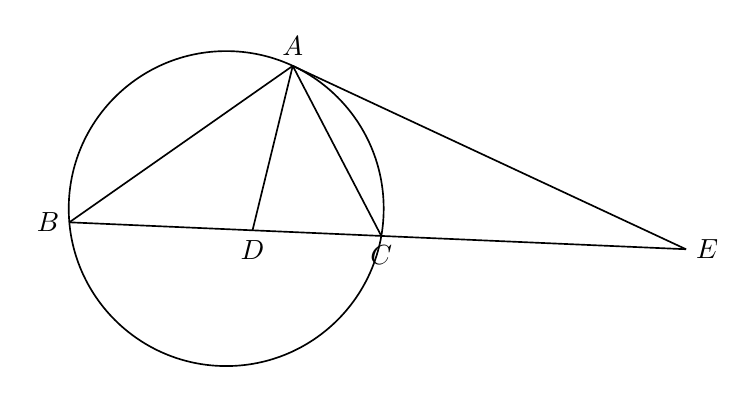
\begin{tikzpicture}[x=1cm,y=1cm,line width=.6pt,font=\normalsize]
\coordinate (O) at (0,0);
\coordinate (A) at (0.8452,1.8126);
\coordinate (B) at (-1.9924,-0.1743);
\coordinate (C) at (1.9696,-0.3473);
\coordinate (D) at (0.3342,-0.2759);
\coordinate (E) at (5.8395,-0.5163);
\draw (O) circle[radius=2cm];
\draw (B)--(E);
\draw (A)--(B);
\draw (A)--(C);
\draw (A)--(D);
\draw (A)--(E);
\node[above] at (A) {$A$};
\node[left] at (B) {$B$};
\node[below] at (C) {$C$};
\node[below] at (D) {$D$};
\node[right] at (E) {$E$};
\end{tikzpicture}
